%% This section adds chapter 4
\section{Background}

\ac{oss} has become a cornerstone of modern software development. It refers to software that is freely available for use, modification, and distribution. The open-source movement has gained significant traction in recent years, driven by a collaborative development philosophy and the benefits it offers to both developers and users.


\subsection{Origins and Early Practices}

The origins of open source software lie in the early days of computing, where a culture of sharing and collaboration thrived. Programmers in academic and research settings freely exchanged and modified code, driven by a desire to improve the technology they worked with. However, as software began to be commercialized, this openness clashed with the rise of proprietary software models. Restrictions on use and a lack of transparency led to frustration among many programmers, sparking the desire for an alternative.

In 1983, Richard Stallman's launch of the GNU Project became a catalyst for the modern open source movement \cite{dibona1999open}.  This ambitious initiative aimed to create a completely free operating system built on the principles of software freedom.  Stallman's advocacy for free redistribution, user modification rights, and transparent development laid the philosophical foundation for the open source movement.

Early open source projects relied heavily on collaborative development through online communities of programmers. This distributed model allowed for efficient bug fixing, rapid development, and fostered knowledge exchange.  Moreover, the creation of licenses like the GNU \ac{gpl} was crucial. These licenses protected open source freedoms, ensuring that software and any modifications made to it would remain accessible to all \cite{license1989gnu}.


Several notable projects defined the early era of open source software. Linus Torvalds' creation of the Linux kernel in 1991 became the poster child for successful open source development, eventually forming the heart of countless operating systems. Additionally, the GNU Project provided essential tools, the Apache Web Server became the dominant force powering the internet, and BIND played a critical role in the internet's infrastructure. These landmark projects proved the viability and potential of the open source model.


\subsection{Defining Open Source}
The definition of open source software is contested. It sparks debate between those who see it as synonymous with "free software" and those who view "open source" as a distinct approach \cite{FuggettaAlfonso2003Osse}.

"Free software", a term stemming from the GNU project, prioritizes user freedoms over cost. At its core, free software grants users the right to use, share, study, modify, and even improve software without restrictions \cite{Whatisfreesoftware}.  Access to the source code is vital, as it is what empowers users to exercise these freedoms.

The term "open source" was introduced later than "free software." While both aim to describe software with accessible source code, there are key philosophical differences. The "open source" term was partly motivated by a desire for a less politically charged, business-friendly label, though its official definition aligns closely with "free software". Stallman argues that the everyday interpretation of "open source" merely denotes visibility of the source code, not the full freedoms of free software \cite{StallmanWhyOpenSource}. This ambiguity allows the term to be applied to semi-free or even proprietary software, diluting its meaning.


While open source initiatives appear in many forms, there are two primary types: open source software and open source content \cite{OregShaul2008Emfc}. Open source software refers to code that is freely available for anyone to inspect, modify, and distribute. This collaborative approach fosters innovation and rapid development. Open source content, on the other hand, encompasses a wider range of creative materials, such as educational resources, scientific data, and artistic works. Like software, open source content licenses permit users to access, share, and modify the materials under specific guidelines.

\subsection{Open Source Project}
An open-source project is a collaborative endeavor where the source code of a software program or application is made freely available to the public. This means that anyone can view, modify, and distribute the code according to the terms of the project's license. Open-source projects typically encourage transparency, community-driven development, and collaboration among developers from diverse backgrounds.

One of the most widely used definitions of open source comes from the Open Source Initiative (OSI), which defines open source software as having a license that meets the following criteria in the figure \ref{fig:osidef}.

\begin{figure}[ht]
    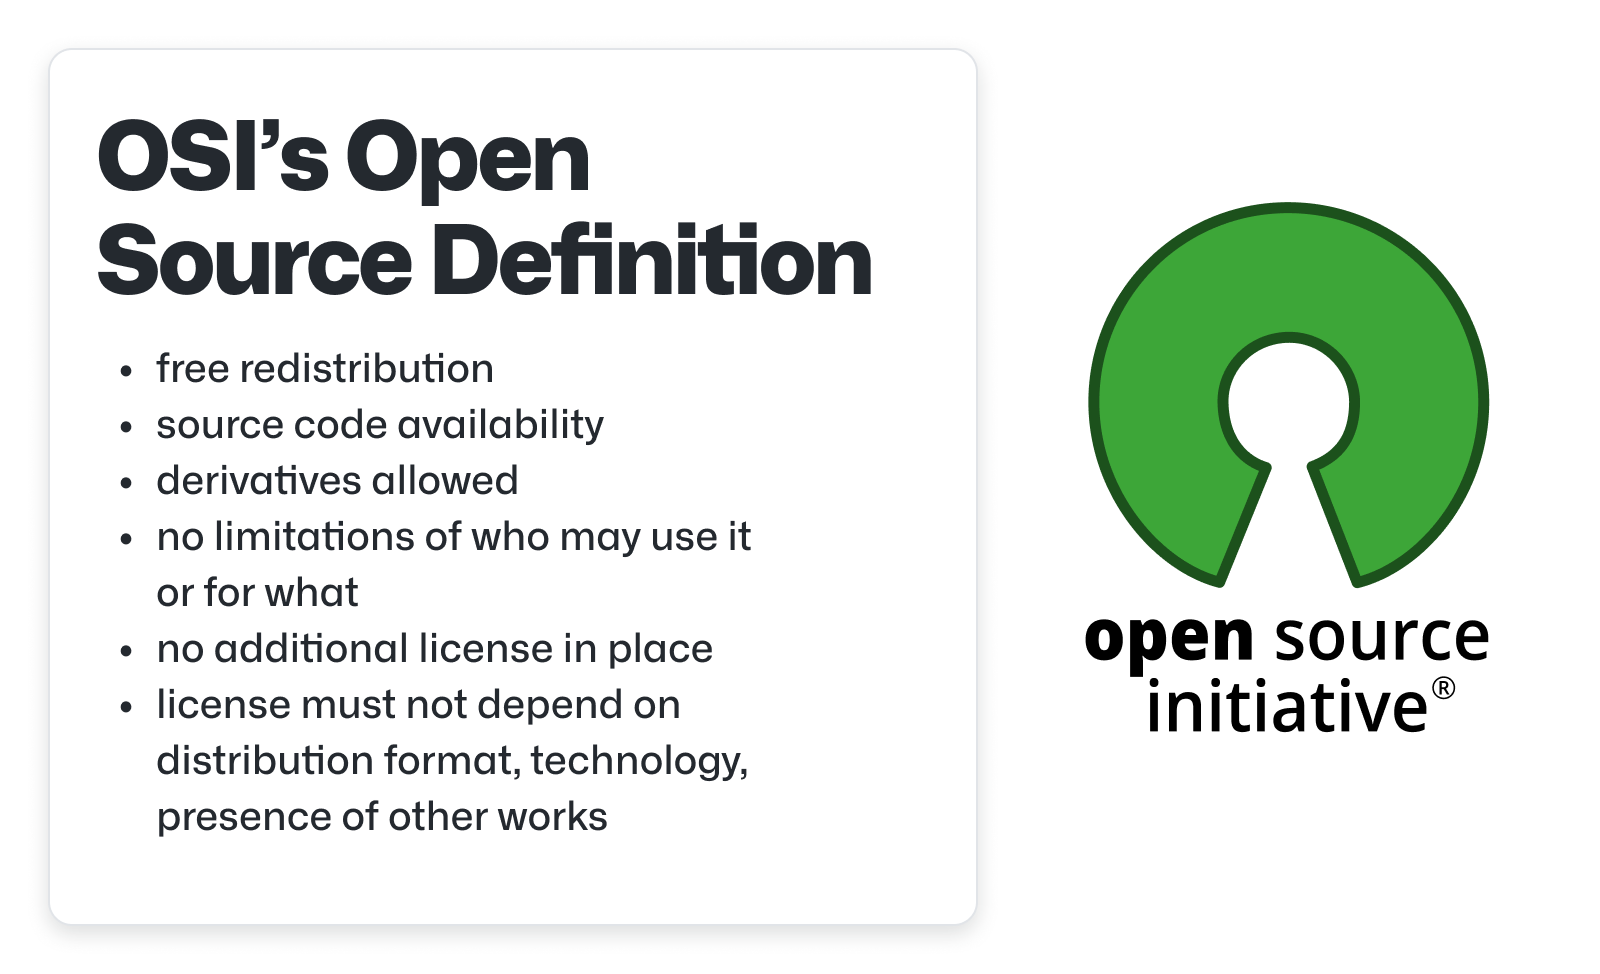
\includegraphics[width=12cm]{figs/osiopensourcedef.png}
    \centering
    \caption{OSI's Open Source Definition \cite{HaeussgeDevGuide}}
    \label{fig:osidef}
\end{figure}



Some of the most popular and influential open-source projects:
\begin{itemize}
    \item Linux: An extremely popular and versatile operating system kernel. Linux powers a vast range of devices from servers and supercomputers to smartphones and embedded systems. It is known for its stability, security, and customization options \cite{fink2003business}.
    \item Git: A distributed version control system that has become the de facto standard for software development. Git allows developers to track changes to code, collaborate easily, and experiment with different branches of development \cite{loeliger2012version}.
    \item Apache HTTP Server: One of the most widely used web server software in the world. It is responsible for serving a significant portion of websites on the internet. Apache is known for its reliability, flexibility, and extensive features \cite{fielding1997apache}.
    \item Python: A high-level, general-purpose programming language that emphasizes readability and ease of use. Python is extremely popular in fields like data science, web development, machine learning, and system administration \cite{srinath2017python}.
    \item TensorFlow: A free, open-source toolset designed to make machine learning accessible. It offers a wide range of tools, libraries, and a supportive community, so both researchers and developers can create and use powerful ML applications \cite{developers2022tensorflow}.
\end{itemize}

\subsection{Ownership and Licensing}

The concept of ownership within the open-source software landscape deviates from the traditional models of individual or corporate proprietorship. While thousands of developers might contribute to a single open-source project, the idea of ownership is more accurately framed in terms of rights, intellectual property, and copyright \cite{Codeownership}.  In this context, it's vital to understand the pivotal role of open-source licenses.

In the world of software, open-source licenses reign supreme. The MIT License offers broad permissions for use, modification, and distribution, making it incredibly developer-friendly \cite{saltzer2020origin}. Similarly, the Apache License 2.0 is permissive and emphasizes providing clear copyright and patent notices \cite{sinclair2010license}. For those seeking "copyleft" protection, ensuring that derived works stay open-source, the GNU \ac{gpl} is a common choice \cite{license1989gnu}.

Licenses establish the boundaries and freedoms granted to users and contributors in utilizing and modifying open-source software \cite{laurent2004understanding}. These licenses come in a variety of forms, each with its own set of rules and restrictions. Some licenses, for example, expressly prohibit the sale of the original software or its derivative versions \cite{madison2003reconstructing}. This is done to safeguard the open-source ethos and prevent commercial exploitation that may stifle community-driven development.

In sum, understanding the intricate interplay of ownership and licensing is essential for navigating the open-source ecosystem. While traditional notions of ownership take a backseat, the principles of intellectual property, copyright, and the specific terms of open-source licenses dictate the rights and responsibilities of all those who interact with this collaborative software model.


\subsection{Morden adoption and future}
\ac{oss} has become a firmly established pillar of the software development landscape, and its influence is poised to grow further in the coming years.  As the open-source community continues to mature and address its challenges, we can anticipate the emergence of even more innovative and powerful solutions driven by this collaborative model.

While the origins of open source can be traced back to the 1960s, with companies like IBM providing free software with their early mainframe systems \cite{moreno2006open}, its widespread adoption has accelerated significantly in recent decades.  Despite the dominance of tech giants like Google, Apple, and Microsoft in the commercial sphere \cite{jacobides2020regulating}, these companies also play a pivotal role in the open-source ecosystem, particularly through contributions on platforms like GitHub.

The substantial impact of open source is exemplified by EU-based companies, which invested an estimated €1 billion in OSS in 2018. This investment yielded a significant return for the European economy, with an estimated contribution ranging from €65 to €95 billion \cite{blind2021impact}.

Figure \ref{fig:bigtechcontributes} underscores the active participation of tech leaders in the open-source movement.  In 2020 alone, 5,709 Google employees submitted over ten commits to GitHub's public code repository.  This was closely followed by contributions from Microsoft, Red Hat, IBM, and others...

\begin{figure}[ht]
    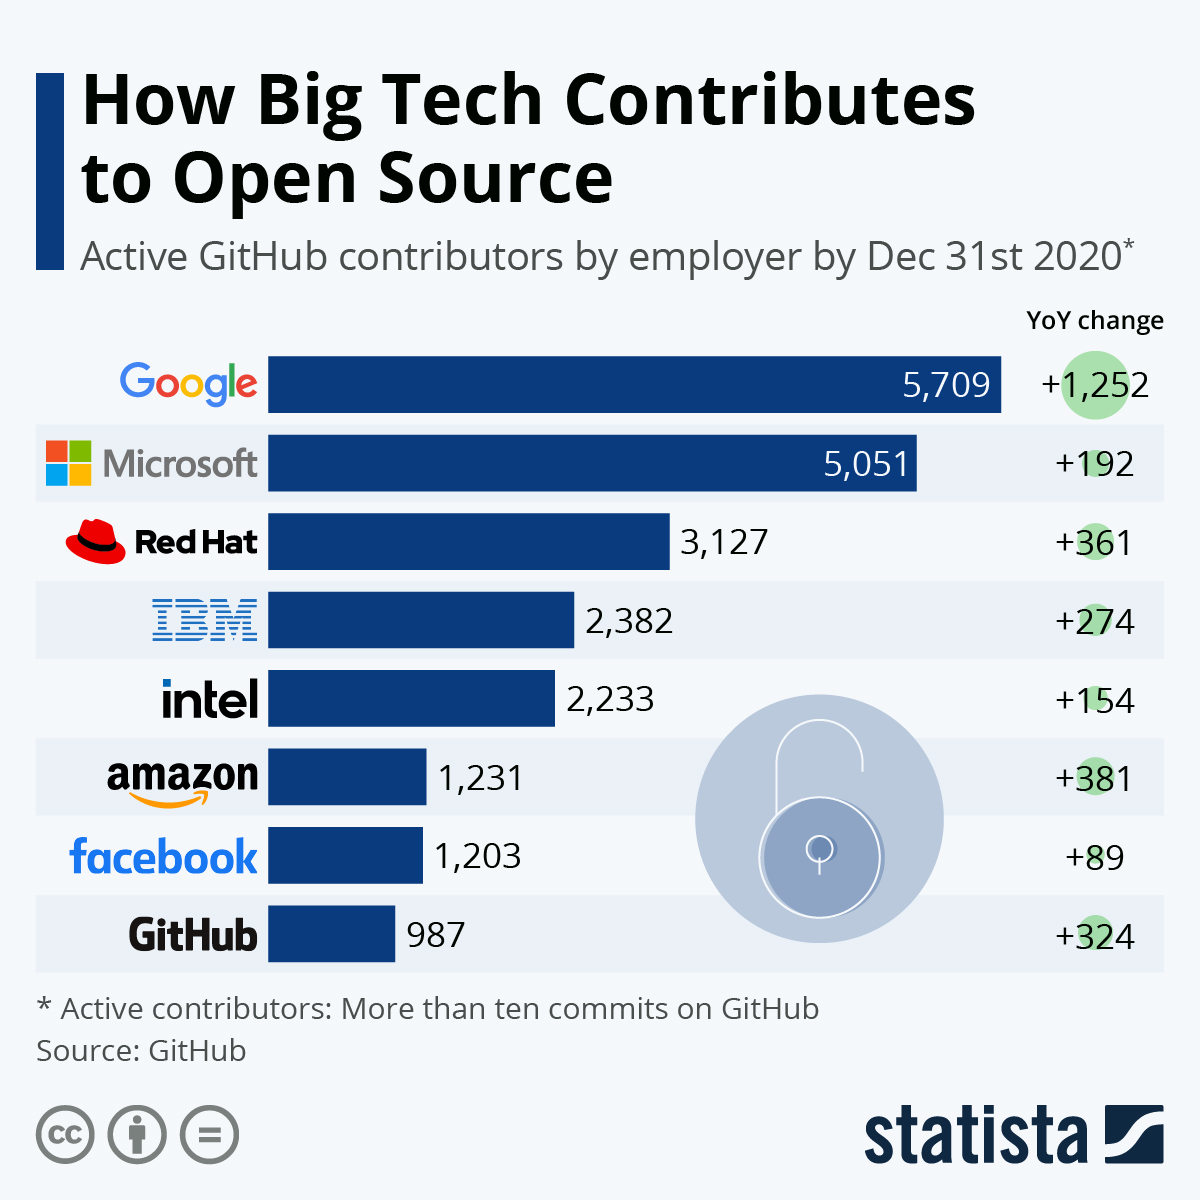
\includegraphics[width=10cm]{figs/bigtechcontributes.jpeg}
    \centering
    \caption{How How Big Tech Contributes to Open Source \cite{statista2021bigtechopensource}}
    \label{fig:bigtechcontributes}
\end{figure}

The open-source movement's trajectory promises transformative impacts across industries, fueled by increasing collaboration, transparency, and knowledge sharing within its expanding community. This trajectory indicates the emergence of groundbreaking technologies, tools, and solutions that will serve the interests of both users and developers, underscoring the potential of open source to revolutionize sectors and drive innovation on a global scale.


\begin{figure}[ht]
    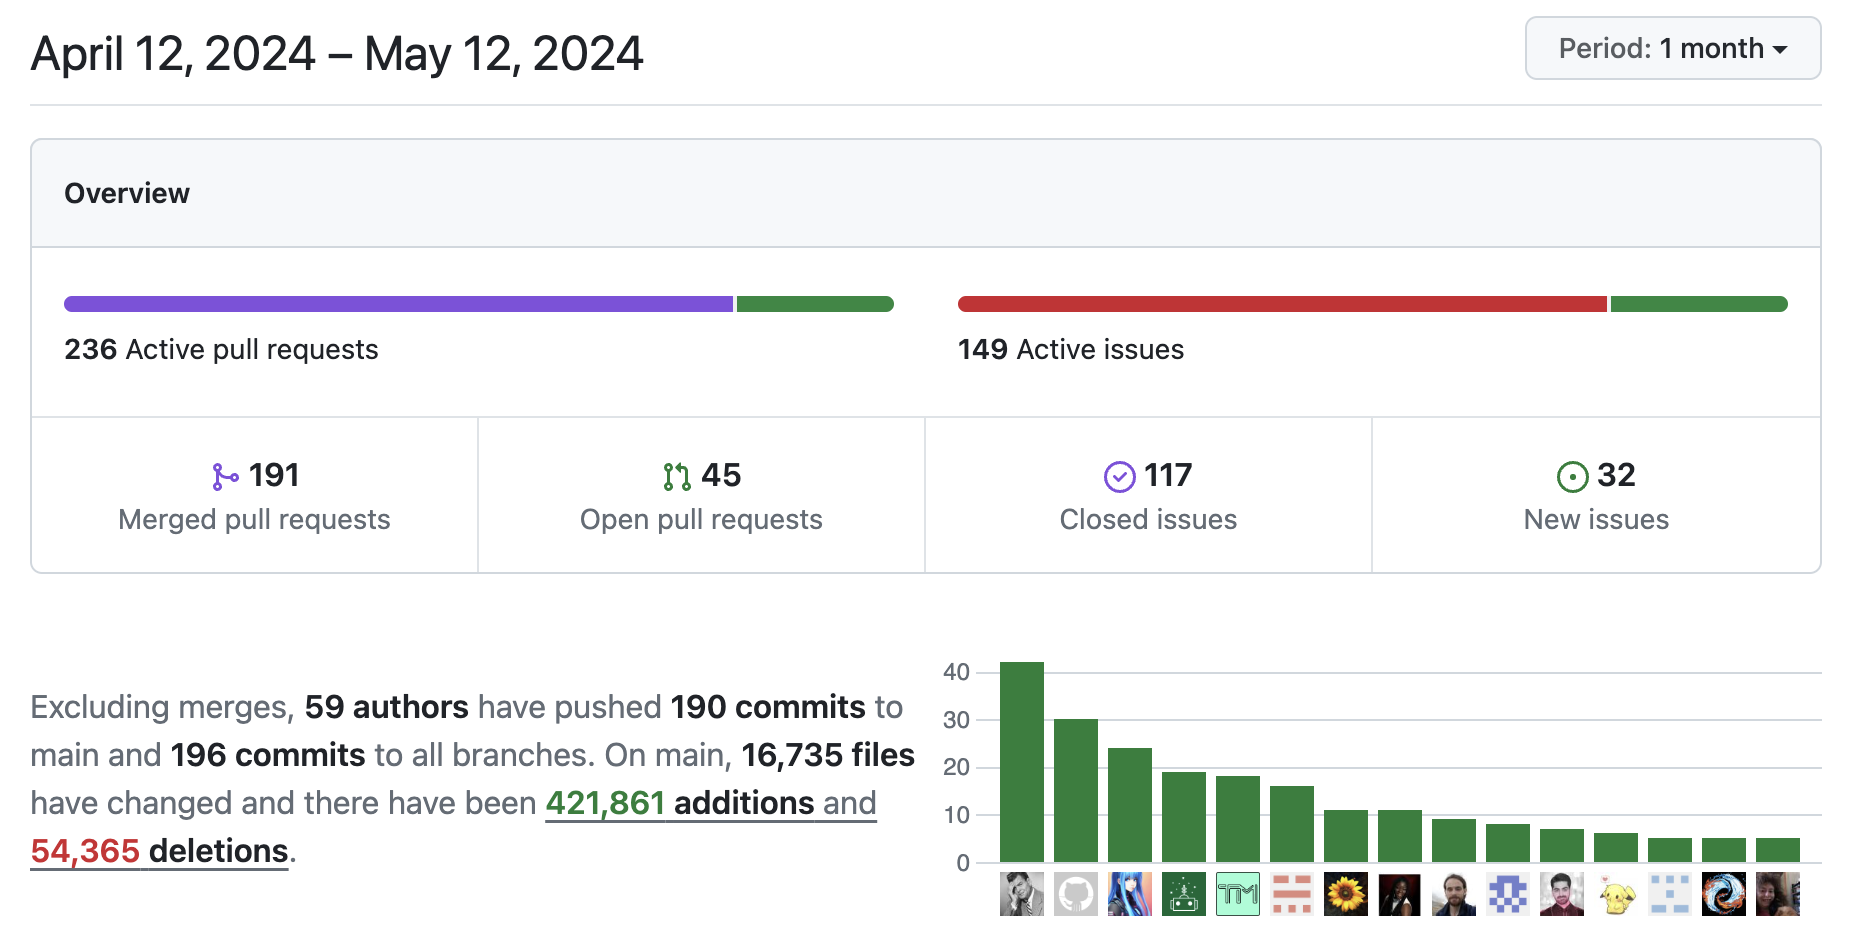
\includegraphics[width=12cm]{figs/freecodecamp.png}
    \centering
    \caption{FreeCodeCamp's Open Source Contribution}
    \label{fig:freeCodeCamp}
\end{figure}




\clearpage  % This command will start the next section from the new page
